% !TEX root = ../paper.tex
\section{Interaction techniques}
The purpose of our experiment is to test different interaction techniques against each other.
Before designing and implementing the experiment we must find a suitable number of techniques to test. 
We decided on four interaction techniques and in this section we describe them and explain why these four techniques were chosen.

Our four techniques all make use of some combination of air pointing and touch gestures on the smartphone screen.
By using the Kinect's depth camera it is possible to facilitate air pointing and when it is combined with a smartphone's touch sensors, it is possible to design different interaction techniques.
However, in this paper we are interested in techniques which have been used in related work. 
We found the techniques in previously published papers where they were used in applications or systems to interact between devices, such as the interaction between a phone and display. 
We name the techniques: \swipe, \tilt, \throw, and \pinch.
\swipe and \tilt are one-handed techniques, meaning they are supposed to be performed with only one hand, opposed to \throw and \pinch which are techniques that require both hands.

The \swipe technique (\Cref*{fig:swipeTechnique}) is used by Bragdon et al. \cite{Bragdon:2011} in Code Space, a system using Kinect and smartphones to support developer meetings. 
Bragdon et al. describes the technique as: \emph{``cross-device interaction with touch and air pointing''} and the swipe motion is described as \emph{``flicking up on the touch screen''}. 
The \swipe technique is performed by 
\begin{enumerate*}[label=\itshape\arabic*\upshape)]
	\item{pointing at a target on the large display with the phone in stretched arm, and}
	\item{making a forwards swipe motion on the phone.}
\end{enumerate*}

The \tilt technique (\Cref{fig:tiltTechnique}) is used in a collaborative application by Lucero et al. \cite{Lucero:2012} to transfer an object from a large display to the user's smartphone.
Boring et al. uses the a tilt technique in \cite{Boring:2009} when moving a pointer on a display using a phone.
The \tilt technique is performed by 
\begin{enumerate*}[label=\itshape\arabic*\upshape)]
	\item{pointing at a target on the large display with the phone in stretched arm, and}
	\item{making a forwards tilt with the phone.}
\end{enumerate*}

\begin{figure}
\subfloat[]{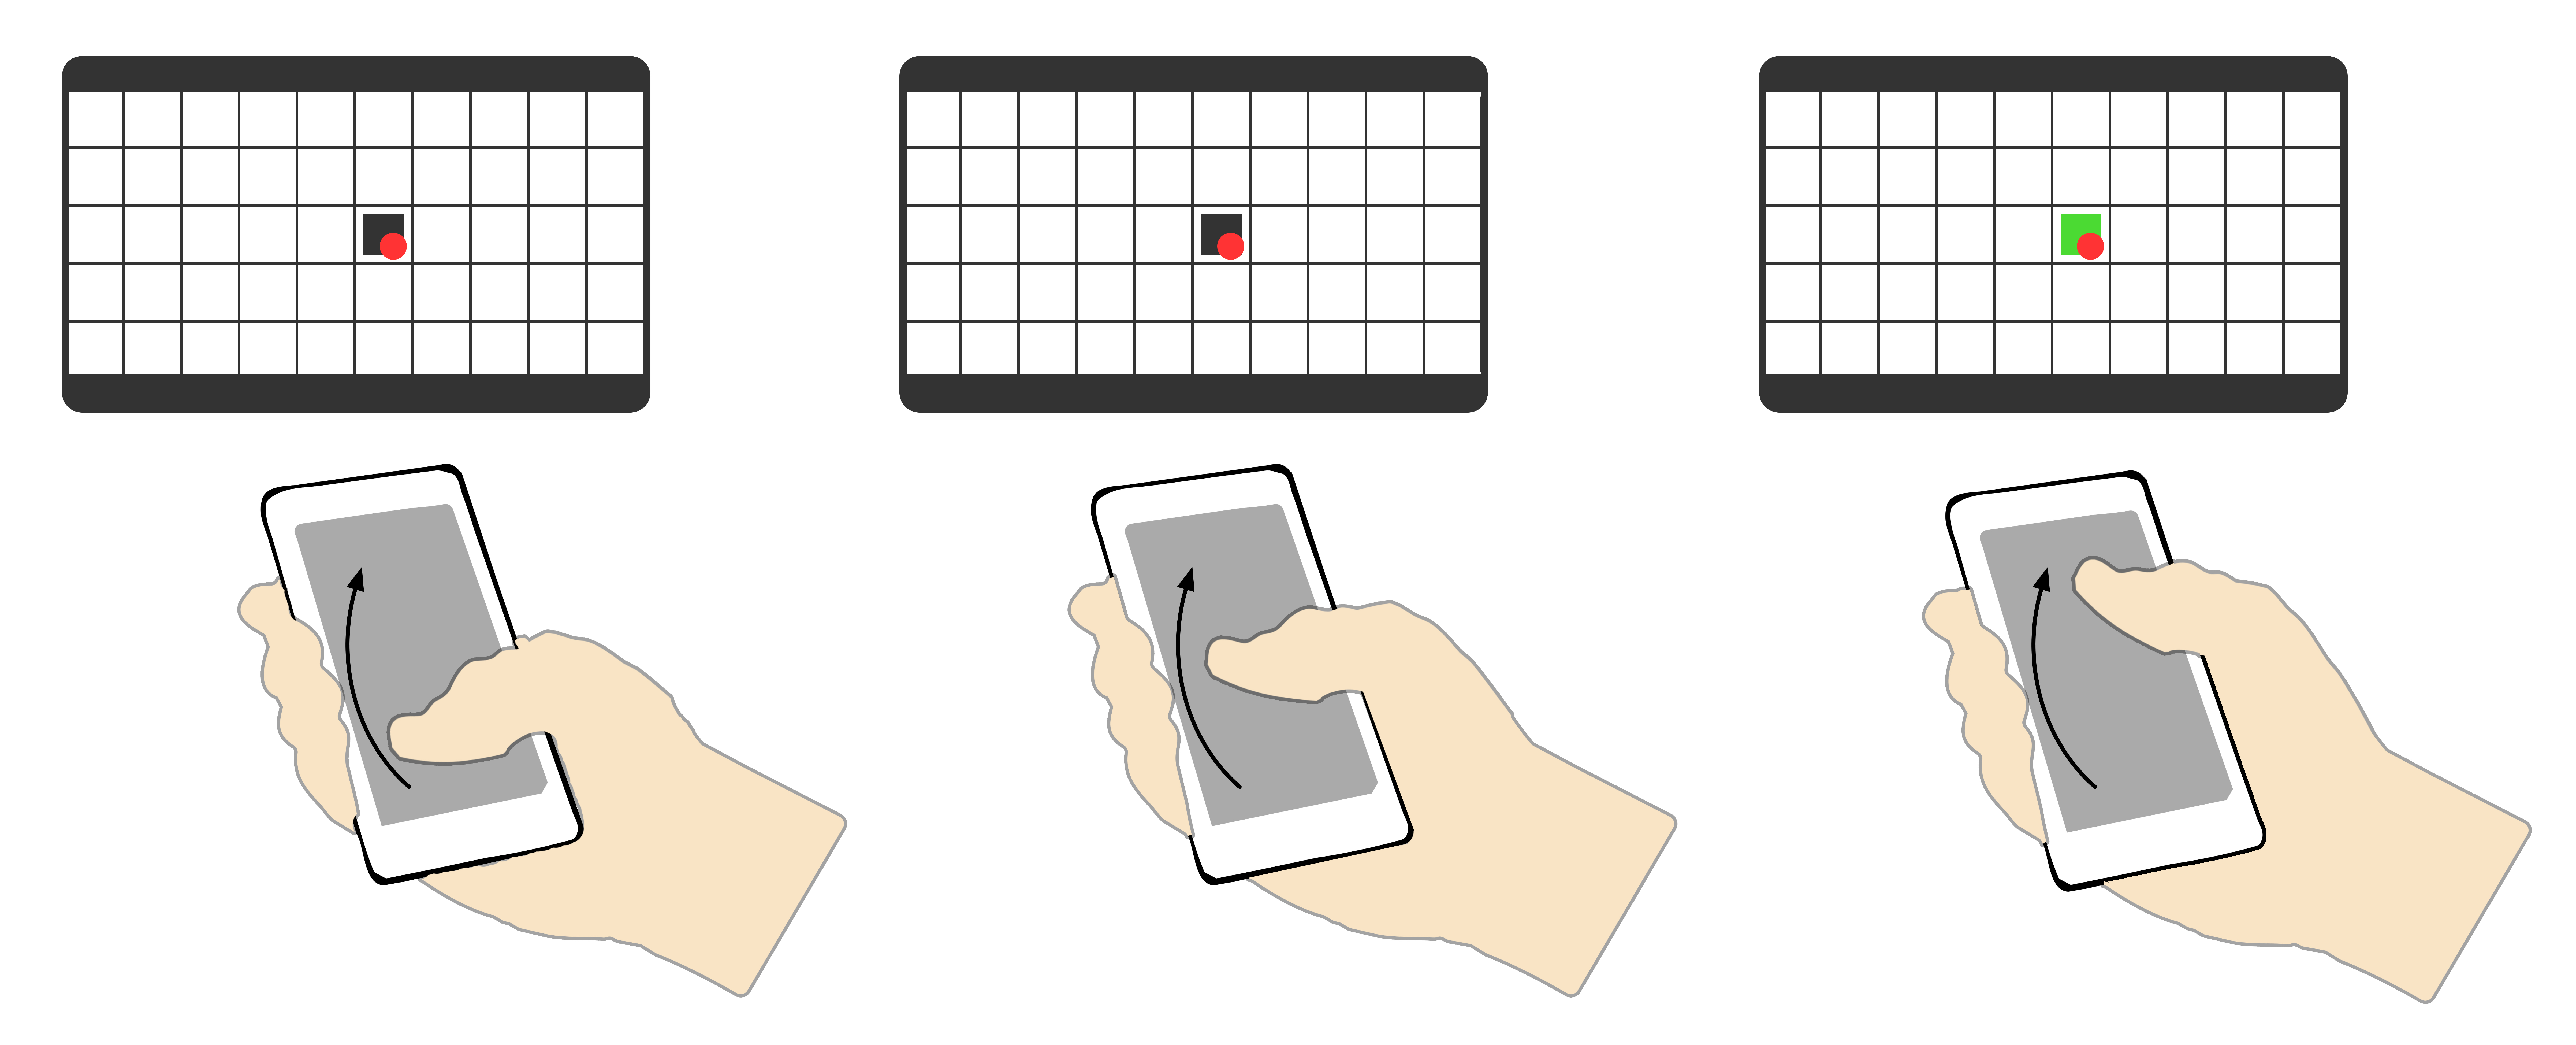
\includegraphics[width = 0.5\columnwidth]{images/swipe.jpg}\label{fig:swipeTechnique}} 
\subfloat[]{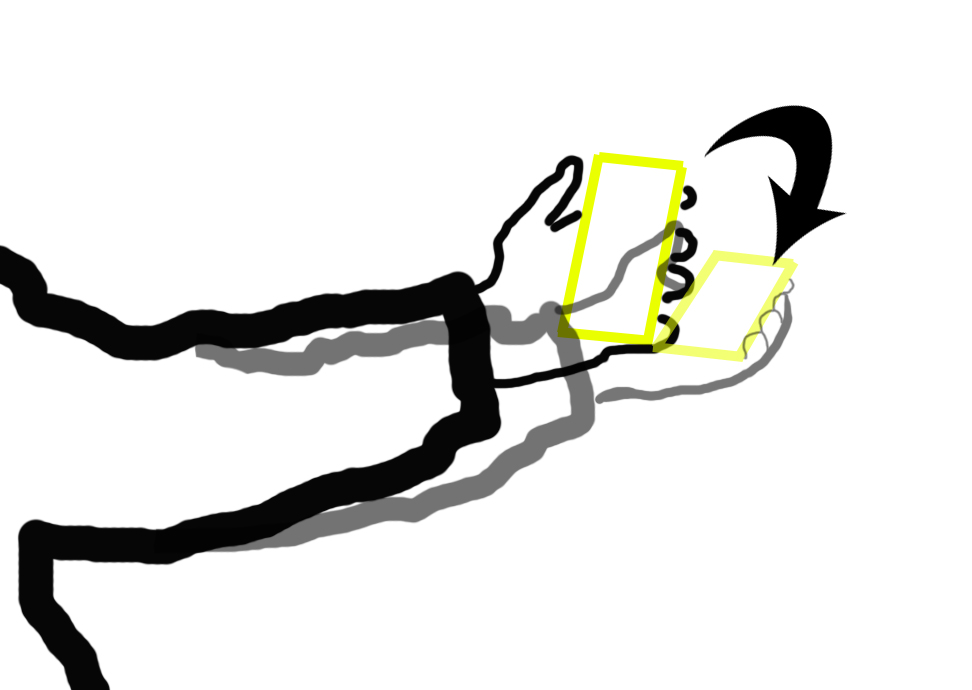
\includegraphics[width = 0.5\columnwidth]{images/tilt.jpg}\label{fig:tiltTechnique}}
\caption{
	\protect\subref{fig:swipeTechnique} swipe technique
	\protect\subref{fig:tiltTechnique} tilt technique
}
\label{fig:swipeTilt}
\end{figure}

The \throw technique (\Cref{fig:throwTechnique}) is a combination of  
\begin{enumerate*}[label=\itshape\alph*\upshape)]
	\item{a technique for pointing \cite{Scheible:2008} i.e. using a hand as a cursor in mid-air, and}
	\item{a throw technique described by Walter et al. \cite{Walter:2014} and used in a system for sharing information on large public displays.}
\end{enumerate*}
The \throw technique is performed by 
\begin{enumerate*}[label=\itshape\arabic*\upshape)]
	\item{pointing at a target on the large display with one hand} 
	\item{holding the phone in the other hand, and}
	\item{making a swinging motion towards the large display.}
\end{enumerate*}

\begin{figure}
\subfloat[]{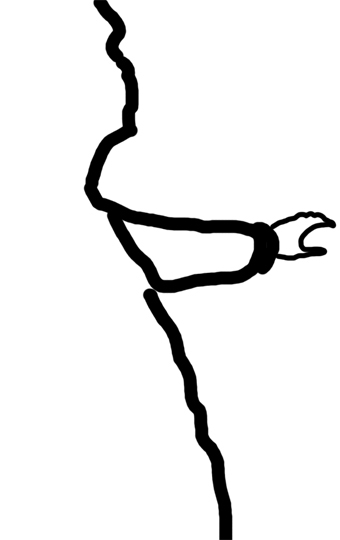
\includegraphics[width = 0.48\columnwidth]{images/throw1.jpg}\label{fig:throwTechnique1}}
\hspace{0.02\columnwidth} 
\subfloat[]{
\includegraphics[width = 0.48\columnwidth]{images/throw2.jpg}\label{fig:throwTechnique2}}
\caption{
	\protect\subref{fig:throwTechnique1} throw technique step1 
	\protect\subref{fig:throwTechnique2} throw technique step2
}
\label{fig:throwTechnique}
\end{figure}

The \pinch technique (\Cref{fig:pinchTechnique}) is used in \cite{Ikematsu:2015} as part of a drag-and-drop method for moving data objects between devices.
Chen et al. uses a pinching gesture in \cite{Chen:2014} for cross-device interaction between a smartphone and a smartwatch. 
In \cite{Benko:2010}, Benko and Wilson used the \pinch technique for interacting with an omnidirectional dome.
The \pinch technique is performed by 
\begin{enumerate*}[label=\itshape\arabic*\upshape)]
	\item{holding the phone in one hand} 
	\item{making a pinch gesture on the phone with the other hand, subsequently closing the hand}
	\item{pointing at a target on the large display with the closed hand, and}
	\item{opening the hand to complete the technique.}
\end{enumerate*}

\begin{figure}
\subfloat[]{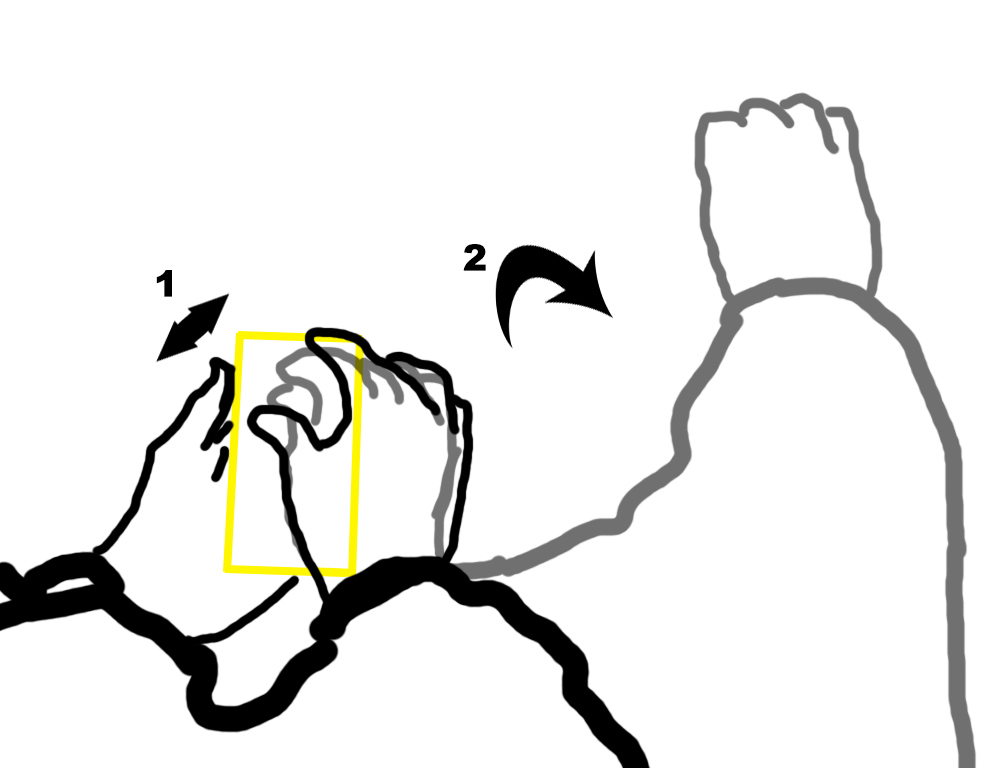
\includegraphics[width = 0.48\columnwidth]{images/pinch1.jpg}\label{fig:pinchTechnique1}}
\hspace{0.02\columnwidth}  
\subfloat[]{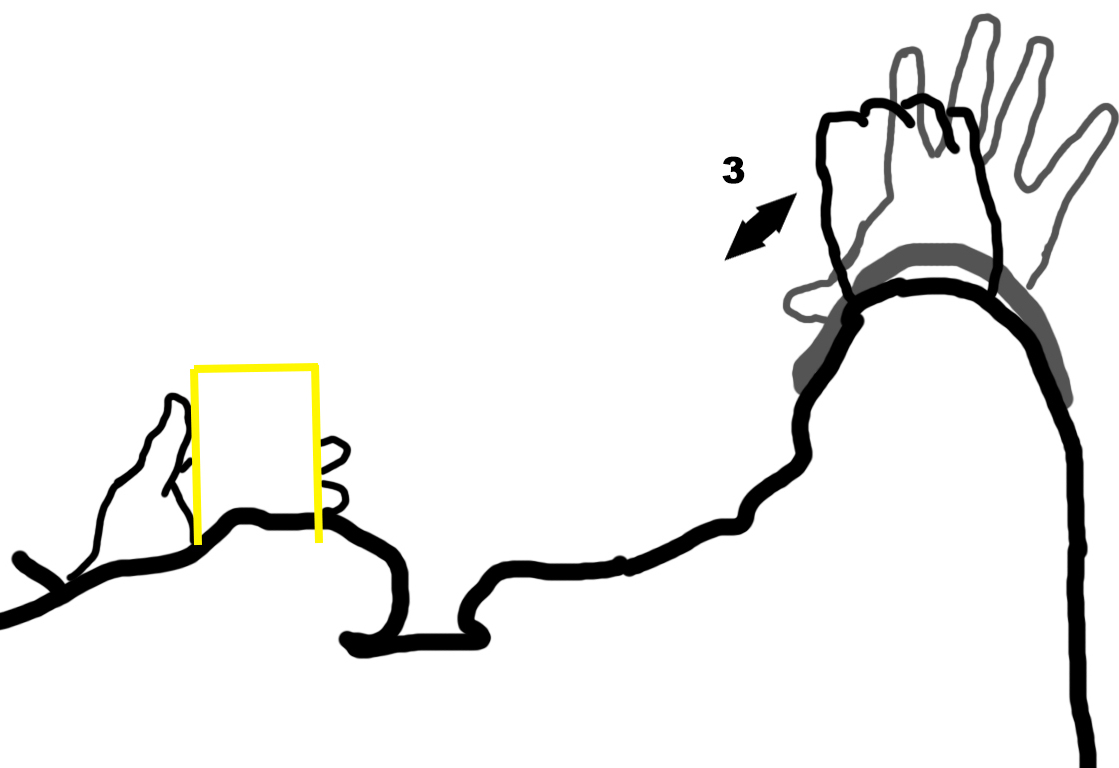
\includegraphics[width = 0.48\columnwidth]{images/pinch2.jpg}\label{fig:pinchTechnique2}}
\caption{
	\protect\subref{fig:pinchTechnique1} pinch technique step1 
	\protect\subref{fig:pinchTechnique2} pinch technique step2
}
\label{fig:pinchTechnique}
\end{figure}